\documentclass[12pt]{article}

\setlength\parindent{0pt}
\newcommand{\myt}[1]{\textbf{\underline{#1}}}

\usepackage{mathtools}
\usepackage{amssymb}
\usepackage{graphicx}

\title{\vspace{-15ex}Math 239 Lecture 22\vspace{-1ex}}
\date{June 29th, 2015}
\author{Graham Cooper}

\begin{document}
	\maketitle
	
	Items:\\
	\begin{itemize}
		\item Bridges
		\item Trees
	\end{itemize}
	
	\section*{Bridges}
	
	\myt{Theorem:} IF e = uv is a bridge of a connected graph G, then G-e has exactly two components. Moreover, u and v are in different components of G-e.\\
	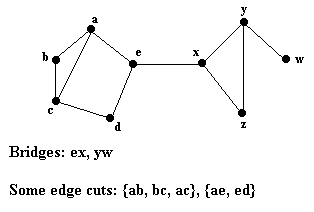
\includegraphics[scale=0.5]{bridge.png}
	
	\myt{Proof:}\\
	(Recall the cut induced by the vertices of a component is empty).\\
	Suppose BWOC that G-e has 3 components. Let H be one component not containing u nor v. The cut induced by V(H) in G-e is empty, but uv is not in the cut induced by V(H) in G, since u,v $\notin$ V(H). So the cut induced by V(H) in G is empty. This contradicts the fact that G is connected.\\
	So G-e has exactly 2 components.\\
	
	Suppose BWOC u,v are in the same component of G-e. Let J be the component. Sothe cut induced by V(J) in G-e is empty. Since u,v $\in$ V(J), e is not in the cut induced by V(J) in G. So this cut is empty in G, contradiction. So u,v are in differnt component of G-e\\
	
	\myt{Theorem:} An edge e = uv in G is a bridge if and only if e is not in any cycle of G.\\
	
	\myt{Contrapositive:} e is in a cycle of G if and only if e is not a bridge.
	
	\myt{Proof: $\implies$}: Suppose that e is in a cycle, u,v,v1,v2....u. Then in G-e, there is a u,v-path v,v1,v2....u. so u,v are in the same component of G-e. Using the contrapositive of the previous theorem, e is not a bridge.
	
	\myt{$\impliedby$} Suppose e is not a bridge. Let H be the component containing e. Then H-e is still connected. So it contains a u,v-path, which does not includ ee. Then P+e is a cycle containing e.
	
	\section*{Trees}
	
	\myt{Definition:} A tree is a connected graph with no cycles.\\
	\myt{Definition:} A forest is a graph with no cycles.\\
	
	\myt{Lemma:} Everye edge in a Tree/Forest is a bridge.\\
	
	\myt{Definition} A leaf in a tree is a vertex of degree 1\\
	
	\myt{Theorem:} Every tree with at least 2 vertices have at least 2 leaves.\\
	\myt{Proof:} Let T be a tree and let P = v0,v1 ... vk be the longest path in T. P has lenght at least 1 since there are $\geq$ 2 vertices. Vertex V0 has one neighbour v1. It cannot have any neighbour outside of P (For otherwise P is not the longest path), nor could it have a neighbour on P other than V1 (otherwise it forms a cycle). So deg(v0)=1 and its a leaf. Sone argument applies to Vk, so T has at least 2 leaves.\\
	
	
	
\end{document}
